% !TEX encoding = UTF-8 Unicode
\documentclass{beamer}

\usepackage[MeX]{polski}
\usepackage[utf8]{inputenc}

\usetheme{Madrid}

\usepackage{graphics}
\usepackage{amsfonts, amssymb, amsmath}

\providecommand{\ar}{\arrow}
\newcommand{\Em}{\mathbb M}


\frenchspacing

\providecommand{\cal}{\mathcal}
\renewcommand{\Bbb}{\mathbb}
\renewcommand{\frak}{\mathfrak}
\newenvironment{pf}{\begin{proof}}{\end{proof}}

%%%%%%%%%%%%%%%%%%%%
% Standard commands
%%%%%%%%%%%%%%%%%%%%

%ᅵᅵᅵᅵᅵᅵᅵᅵᅵᅵᅵᅵᅵᅵᅵᅵ
% Caligraphic and bold letters. 
%ᅵᅵᅵᅵᅵᅵᅵᅵᅵᅵᅵᅵᅵᅵᅵᅵᅵ
\newcommand{\Aa}{{\Bbb{A}}}
\newcommand{\Aaa}{{\cal{A}}}
\newcommand{\Bee}{{\cal{B}}}
\newcommand{\Cee}{{\cal{C}}}
\newcommand{\Dee}{{\cal{D}}}
\newcommand{\Ef}{{\cal{F}}}
\newcommand{\Gee}{{\cal{G}}}
\newcommand{\Haa}{{\cal{H}}}
\newcommand{\Ai}{\cal{I}}
\newcommand{\Kay}{{\cal{K}}}
\newcommand{\El}{{\cal{L}}}
\newcommand{\Pee}{{\cal{P}}}
\newcommand{\See}{{\cal{S}}}
\newcommand{\Tau}{{\cal{T}}}
\newcommand{\Yu}{{\cal{U}}}
\newcommand{\Vee}{{\cal{V}}}
\newcommand{\Wu}{{\cal{W}}}
\newcommand{\Zee}{{\Bbb{Z}}}
\newcommand{\Emm}{{\frak{M}}}
\newcommand{\Be}{{\Bbb{B}}}
\newcommand{\Nat}{{\Bbb{N}}}
\newcommand{\Z}{{\mathbb Z}} % The integers
\newcommand{\Qyu}{{\Bbb{Q}}}
\newcommand{\Err}{{\Bbb{R}}}


%ᅵᅵᅵᅵᅵᅵᅵᅵᅵᅵᅵᅵᅵᅵᅵᅵᅵᅵ
% Shortcuts for some Greek letters. 
%ᅵᅵᅵᅵᅵᅵᅵᅵᅵᅵᅵᅵᅵᅵᅵᅵᅵᅵᅵ
\newcommand{\lam}{{\lambda}}
\newcommand{\al}{\alpha}
\newcommand{\Gam}{\Gamma}
\newcommand{\alG}{\al\in\Gamma}
\newcommand{\sig}{\sigma}
\newcommand{\eps}{\varepsilon}
\renewcommand{\phi}{\varphi}
\renewcommand{\rho}{\varrho}


%ᅵᅵᅵᅵᅵᅵᅵᅵᅵ
% Basic commands. 
%ᅵᅵᅵᅵᅵᅵᅵᅵᅵᅵ
\newcommand{\rest}{\restriction}
\newcommand{\unii}{\mathbb I}
\newcommand{\ntr}{{n\in\omega}}
\newcommand{\Ntr}{n\in{\Bbb{N}}}
\newcommand{\loe}{\leq}
\newcommand{\goe}{\geq}
\newcommand{\notloe}{\nleq}
\newcommand{\notgoe}{\ngeq}
\newcommand{\subs}{\subseteq}
\newcommand{\sups}{\supseteq}
\newcommand{\nnempty}{\ne\emptyset}
\newcommand{\argum}{\:\cdot\:}
\newcommand{\ovr}{\overline}
\renewcommand{\iff}{\Longleftrightarrow}


%ᅵᅵᅵᅵᅵᅵ
% Topology. 
%ᅵᅵᅵᅵᅵᅵᅵ
\newcommand{\Cl}[1]{\overline{#1}}
\newcommand{\cl}{\operatorname{cl}}
\newcommand{\Int}{\operatorname{int}}
\newcommand{\w}{\operatorname{w}}
\newcommand{\dens}{\operatorname{dens}}
\newcommand{\eXp}{\operatorname{exp}}
\newcommand{\diam}{\operatorname{diam}}
\newcommand{\dist}{\operatorname{dist}}
\newcommand{\nbd}{\operatorname{nbd}}



%ᅵᅵᅵᅵᅵᅵĿ
% Convexity. 
%ᅵᅵᅵᅵᅵᅵᅵ
\newcommand{\conv}{\operatorname{conv}}
\newcommand{\co}{\operatorname{co}}
\newcommand{\clco}{\operatorname{clco}}
\newcommand{\m}{\operatorname{m}}
\newcommand{\med}{\operatorname{med}}

\newcommand{\G}{{\mathbb G}}

%ᅵᅵᅵᅵᅵᅵᅵᅵ
% Miscellanous. 
%ᅵᅵᅵᅵᅵᅵᅵᅵᅵ
\newcommand{\id}[1]{{\operatorname{i\!d}_{#1}}} % identity morphism
\newcommand{\cf}{\operatorname{cf}}
\newcommand{\dom}{\operatorname{dom}}
\newcommand{\cod}{\operatorname{cod}}
\newcommand{\Dom}{\operatorname{Dom}}
\newcommand{\rng}{\operatorname{rng}}
\newcommand{\suppt}{\operatorname{suppt}}
\newcommand{\defi}{\stackrel{\rm df}=}
\newcommand{\pr}{\operatorname{pr}}
\newcommand{\liminv}{\varprojlim}

\newcommand{\symd}{\div} % <--- Symmetrical difference

\newcommand{\oraz}{\qquad\text{and}\qquad}

%ᅵᅵᅵᅵᅵᅵᅵᅵᅵᅵᅵᅵĿ
% Some forcing commands. 
%ᅵᅵᅵᅵᅵᅵᅵᅵᅵᅵᅵᅵᅵ
\newcommand{\proves}{\vdash}
\newcommand{\forces}{\Vdash}
\newcommand{\Con}{\operatorname{Con}}
\newcommand{\Card}{{\frak{Card}}}
\newcommand{\Func}{\operatorname{Func}}
\newcommand{\rank}{\operatorname{rank}}
\newcommand{\poset}{{\Bbb{P}}}
\newcommand{\Forall}{\forall\;}
\newcommand{\Exists}{\exists\;}
\newcommand{\h}{\widehat}
\newcommand{\val}{\operatorname{val}}
\newcommand{\comp}{\parallel}
\newcommand{\incomp}{\perp}
\newcommand{\Es}{{\cal{S}}}
\newcommand{\meet}{\wedge}
\newcommand{\Meet}{\prod}
\newcommand{\join}{\vee}
\renewcommand{\Join}{\sum}
\newcommand{\Land}{\;\&\;}


%ᅵᅵᅵᅵĿ
% Trees. 
%ᅵᅵᅵᅵᅵ
\newcommand{\Lev}{\operatorname{Lev}}
\newcommand{\lev}[2]{{\ell_{#1}#2}}
\newcommand{\Ht}{\operatorname{ht}}
\newcommand{\length}{\operatorname{length}}
\newcommand{\bd}{\partial}

\newcommand{\concat}{{}^\smallfrown}
\newcommand{\Reg}{{\frak{Reg}}}
\newcommand{\Ord}{{\frak{Ord}}}
\newcommand{\by}[1]{/_{#1}}
\newcommand{\club}{\operatorname{club}}
\newcommand{\proj}{\operatorname{proj}}
\newcommand{\otp}{\operatorname{otp}}
\newcommand{\Fin}{\operatorname{fin}}

%ᅵᅵᅵᅵᅵᅵᅵᅵᅵᅵᅵᅵᅵ
% Theorems and Propositions. 
%ᅵᅵᅵᅵᅵᅵᅵᅵᅵᅵᅵᅵᅵᅵᅵ
\newtheorem{tw}{Theorem}[section]
\newtheorem{wn}[tw]{Corollary}
\newtheorem{lm}[tw]{Lemma}
\newtheorem{prop}[tw]{Proposition}
\newtheorem{claim}[tw]{Claim}
\theoremstyle{definition}
\newtheorem{df}[tw]{Definition}
\newtheorem{ex}[tw]{Example}
\newtheorem{pyt}[tw]{Question}
\newtheorem{question}[tw]{Question}
\theoremstyle{remark}
\newtheorem{uwgi}{Remark}
\renewcommand{\theuwgi}{}

\newcommand{\setd}[2]{\{#1,\dots,#2\}}
\newcommand{\set}[1]{\{#1\}}
\newcommand{\setof}[2]{\{#1\colon #2\}}
\newcommand{\bigsetof}[2]{\Bigl\{#1\colon #2\Bigr\}}
\newcommand{\seq}[1]{\langle #1 \rangle}
\newcommand{\seqof}[2]{\langle #1\colon #2\rangle}
\newcommand{\sett}[2]{\{#1\}_{#2}}
\newcommand{\sn}[1]{\{#1\}} % singleton
\newcommand{\dn}[2]{\{#1,#2\}} % doubleton
\newcommand{\pair}[2]{\langle #1, #2 \rangle} % pair
\newcommand{\triple}[3]{\langle #1, #2, #3 \rangle} % triple
\newcommand{\map}[3]{#1\colon #2 \to #3} % A function
\newcommand{\img}[2]{#1[#2]} % image of a set
\newcommand{\inv}[2]{{#1}^{-1}[#2]} % preimage of a set


% Cantor's stuff:
\newcommand{\Cantor}{2^\omega}


% added 19 March 2002
\newcommand{\power}[1]{\Pee(#1)}
\newcommand{\dpower}[2]{[#1]^{#2}}
\newcommand{\truj}[1]{{\dpower{#1}{\loe2}}}
\newcommand{\fin}[1]{[#1]^{<\omega}}
\newcommand{\finom}{\fin \omega}

\newcommand{\fra}{Fra\"iss\'e}
\newcommand{\jon}{J\'onsson}
\newcommand{\frajon}{\fra-\jon}
\newcommand{\U}{\mathbb U}
\newcommand{\M}{\mathbb M}
\newcommand{\bL}{{\mathbb L}}
\newcommand{\Ama}{{\mathcal A}} % Amalgamation structure

%\newcommand{\f}{{fin}}

\providecommand{\nat}{\omega}
\newcommand{\setind}[2]{\sett{{#1}_{#2}}{{#2}\in\nat}}
\newcommand{\ciag}[1]{{\sett{{#1}_n}{\ntr}}}


% added 17 March 2005
% Categories:
\newcommand{\dualcat}[1]{{\ensuremath{{#1}^{\operatorname{op}}}}}
\newcommand{\mor}{\operatorname{Mor}}
\newcommand{\ind}[2]{\triple{{#1}_n}{{#2}_n^m}{\omega}}
\newcommand{\indi}[4]{\triple{{#1}_{#3}}{{#2}_{#3}^{#4}}{\omega}}
\newcommand{\aut}{\operatorname{Aut}}
\newcommand{\End}{\operatorname{End}}
\newcommand{\flim}{\operatorname{Flim}}
\newcommand{\Arr}{\operatorname{Arr}}
\newcommand{\ob}{\operatorname{Obj}}
\newcommand{\iso}{\approx}
\newcommand{\uzup}[2]{{{\operatorname{Seq}}_{<{#1}}{\left(#2\right)}}}
\newcommand{\uzupiso}[2]{{{\operatorname{Seq}}^{\rm{iso}}_{<{#1}}{\left(#2\right)}}}
\newcommand{\uzuple}[2]{{{\operatorname{Seq}}_{\loe{#1}}{\left(#2\right)}}}


\newcommand{\ciagi}[1]{\sig{#1}}
\newcommand{\mon}[1]{{{}^{\operatorname{mon}}{#1}}}
\newcommand{\epi}[1]{{{}^{\operatorname{epi}}{#1}}}

\newcommand{\emb}[1]{{{}^{\operatorname{e}}{#1}}}
\newcommand{\quo}[1]{{{}^{\operatorname{q}}{#1}}}


\newcommand{\anorm}{\|\cdot\|}
\newcommand{\norm}[1]{\|#1\|}
\newcommand{\bnorm}[1]{\Bigl\|#1\Bigr\|}
\newcommand{\aabs}{|\cdot|}
\newcommand{\abs}[1]{|#1|}
\newcommand{\uball}[1]{\clbal_{#1}}
\newcommand{\ubal}{\uball}
\newcommand{\usphere}[1]{\operatorname{S}_{#1}}


\newcommand{\fK}{{\mathfrak{K}}}
\newcommand{\fL}{{\mathfrak{L}}}
\newcommand{\fM}{{\mathfrak{M}}}
\newcommand{\fC}{{\mathfrak{C}}}
\newcommand{\fS}{{\mathfrak{S}}}
\newcommand{\fT}{{\mathfrak{T}}}
\newcommand{\fU}{{\mathfrak{U}}}
\newcommand{\fB}{{\mathfrak{B}}}



\newcommand{\bS}{{\mathbb{S}}}
\newcommand{\bT}{{\mathbb{T}}}
\newcommand{\bR}{{\mathbb{R}}}
\newcommand{\bU}{{\mathbb{U}}}
\newcommand{\bV}{{\mathbb{V}}}
\newcommand{\bX}{{\mathbb{X}}}
\newcommand{\bY}{{\mathbb{Y}}}

\newcommand{\cmp}{\circ} % composition!!!
\newcommand{\pcmp}{\bullet} % path composition!!!


\newcommand{\invsys}[5]{\langle {#1}_{#4};{#2}_{#4}^{#5};#3 \rangle}

%%% CATEGORIES:
\newcommand{\bdl}{\ensuremath{\mathfrak D\!\!\mathfrak L}} % bounded distributive lattices
\newcommand{\komp}{\ensuremath{\mathfrak C\mathfrak o\mathfrak m\mathfrak p}} % the category of compacta
\newcommand{\mkomp}{\ensuremath{\komp_{\aleph_0}}} % metric compacta
\newcommand{\linkomp}{\ensuremath{\mathfrak L\!\mathfrak c\mathfrak m}} % the category of linearly ordered compacta
\newcommand{\rp}[1]{{\ddag{#1}}} % the category of retractive pairs
\newcommand{\retr}[1]{{{\dag}{#1}}}
\newcommand{\sets}{\ensuremath{\mathfrak S\mathfrak e\mathfrak t}} % the category of sets
\newcommand{\banach}{\ensuremath{\mathfrak B}} % Banach spaces
\newcommand{\sban}{\ensuremath{\banach_{\aleph_0}}} % Separable B-spaces
\newcommand{\sbaniso}{\ensuremath{\banach_{\aleph_0}^{\operatorname{iso}}}} % Separable B-spaces
\newcommand{\LO}{\ensuremath{\mathfrak L\!\mathfrak O}}
\newcommand{\Quna}{\ensuremath{\Qyu_{\omega_1}}} % The uncountable rationals.

\newcommand{\Pel}{\mathbf P}


\newcommand{\sret}{{\mathfrak R}_{\mathcal T}}
\newcommand{\ret}{{\mathfrak R}^{\iso}_{\mathcal T}}

\newcommand{\cont}{\ensuremath{\mathfrak c}}

\newcommand{\trees}{\ensuremath{\mathfrak{T}_2}}
\newcommand{\lord}{\ensuremath{\mathfrak L\mathfrak O_{\aleph_0}}}
\newcommand{\lordli}{\ensuremath{\lord^{\operatorname{li}}}}
\newcommand{\wek}[1]{{\vec{#1}}}
\newcommand{\metapp}{\ensuremath{\mathfrak a\!\mathfrak p\!\mathfrak p\!\mathfrak M}} % metric approximations
\newcommand{\lat}{{\ensuremath \mathfrak L}}
\newcommand{\C}{{\ensuremath\mathcal C}} % The "continuous functions" functor.

\newcommand{\separator}{\begin{center} \leafright \leafright \leafright \decotwo \decotwo \decotwo \leafleft \leafleft\leafleft
\end{center}}

\newcommand{\arrows}[1]{#1(\rightarrow)}
\newcommand{\fun}[3]{{\mathfrak{f}\left(#1,#2, #3 \right)}}
\newcommand{\pref}[2]{\mathcal{P}\left(#1,#2\right)}

\newcommand{\qlim}{{\mathcal L}}
\newcommand{\cocones}[1]{\Delta\left(#1\right)}
\newcommand{\coconesiso}[1]{\Delta^{\rm{iso}}\left(#1\right)}

\newcommand{\bombing}{\bomb\bomb\bomb\bomb\bomb\bomb\bomb\bomb}


\newcommand{\sz}{\ominus}

\newcommand{\zbiry}[1]{{\mathfrak S}_{#1}}



\title[Chord diagrams category]{The category of chord diagrams and its generic limit}
\subtitle{33rd Summer Conference on Topology and its Applications}
\author[S. Zajac and W. Kubis ]{Sebastian Zając \\(joint work with Wieslaw Kubis)}
\institute[UKSW]{Cardinal Stefan Wyszynski University in Warsaw }
\date{20.07.2018}

\begin{document}

\frame{\titlepage}

\section[Outline]{}
\frame{\tableofcontents}

%  At the beginning I want thanks organizers for  give me opportunities to speak at this conference. 
% I want present some beginning work about some special category called a chord diagram category and how to use it with Fraisse theory.
% the schedule of my talk will be devided by two part. At first I show You motivation why it could be interesting and useful and the second one will be about definition of chord diagram category
%
\section{Motivation}

%  slajd 1
\frame
{
  \frametitle{Motivation}
  \begin{block}{}
 Chord diagrams may be used to represent the inter-relationships between some objects. 
\end{block}
\begin{block}{
What is a chord diagram  ? }
Let's consider \texttt{a collection of} $b\geqslant 1$ (pairwise, disjoint, oriented and labeled) \texttt{intervals} lying in the real line. We call them {\tt backbones}. \\ By a {\tt chord diagram} on backbones we understand a collection of $n \geqslant 0$ semi-circles (called {\tt chords}) whose endpoints lie at distinct interior points of backbones.
\end{block}

 
}

% Chord diagrams are very simple things. 
%
%
%



% slajd obrazek diagramu w dwoch postaciach 
\frame{\frametitle{Graphical representation}

\begin{center}
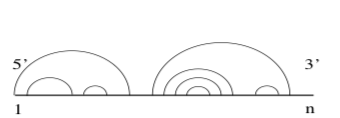
\includegraphics[scale=0.55]{figure1.png}
\newline
\newline
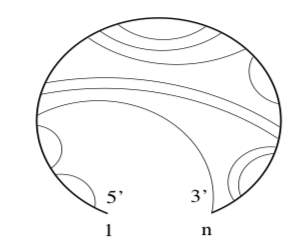
\includegraphics[scale=0.4]{fig2.png}
\newline
\end{center}

\tiny{
T. Doslic ''Secondary structures and some related combinatorial objects'', DOI: https://doi.org/10.5592/CO/CCD.2016.02}
}
% slajd 2 Fizyka
\frame{\frametitle{Where can you find it ?}
\begin{block}{Physics}
\begin{center}
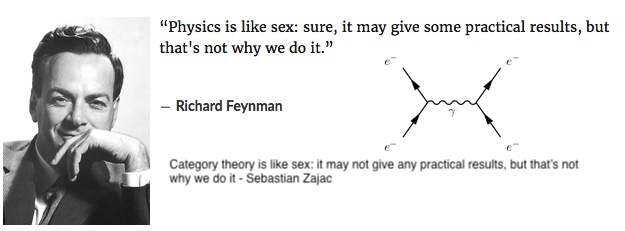
\includegraphics[scale=0.45]{richard.png}
\end{center}
\end{block}
\begin{block}{Math}
\begin{itemize}
\item Matrix Field Theory (0-dim quantum field theory),
\item geometry, topology, representation theory,
\item moduli spaces of Riemann surfaces. 
\end{itemize}
\end{block}

}


% slajd RNA
\frame{
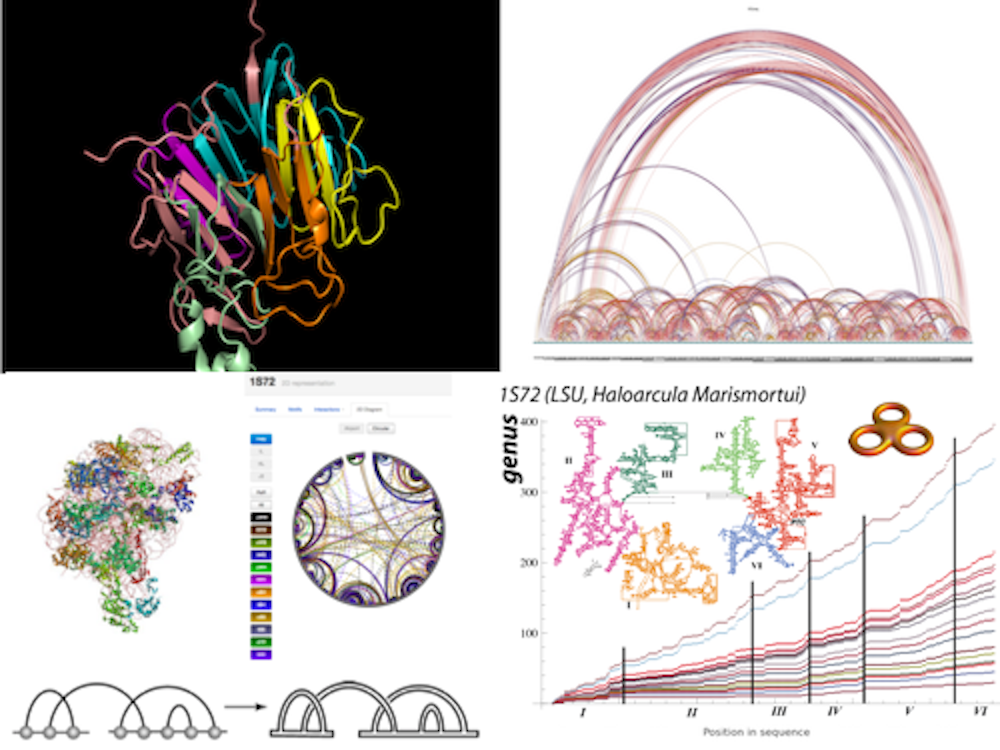
\includegraphics[scale=0.47]{protein.png}
}

\section{The category of chord diagrams}

\frame{\frametitle{Preliminaries}
\begin{enumerate}
\item A natural number $n$ is the set $\{0,1, \dots, n-1\}$.
\item Recall that a \emph{linear ordering} on a set $S$ is an irreflexive transitive relation $<$ satisfying $x < y$ or $y < x$ for every $x \ne y$ in $S$.  In that case $\pair S <$ is called a \emph{linearly ordered} set.
\item If $\pair S {<^S}$ and $\pair T {<^T}$ are linearly ordered sets then a mapping $\map f S T$ is called \emph{increasing} if $f(x) <^T f(y)$ whenever $x <^S y$.
\item If $A, B$ are subsets of a linearly ordered set $\pair{S}{<}$ then we write $A < B$ if $a < b$ holds for every $a \in A$ and $b \in B$.
\item we denote by $\power{S}$ - power-set of $S$ (the set of all subsets of $S$).
\item Given a natural number k, we denote by $[S]^k$ the family of all k- element subsets of S
\item A family $\Aaa \subs \power{S}$ is called a \emph{partition} of $S$ if $S = \bigcup \Aaa$ and $A_0 \cap A_1 = \emptyset$ for every $A_0 \ne A_1$ in $\Aaa$.
\item A \emph{graph} (more formally: a simple undirected graph) is a structure of the form $\pair S E$, where $E \subs \dpower S 2$.
\end{enumerate}
}
% slajd 4 definicja kategorii chordow
\frame{
\frametitle{The category of chord diagrams}
%
We fix three positive integers $k$, $\ell$, and $m$ and a multifunction $$\map{\phi}{\ell \times \ell}{m}$$

The objects of $\fC_{k,\phi}$ are structures of the form
$$\bS = \seq{S, <^S, \sett{B_i^S}{i<k}, \sett{N_i^S}{i<\ell}, \sett{E_i}{i<m}},$$
where:
\begin{enumerate}[itemsep=-2pt]
	\item[(D1)] $\pair{S}{<^S}$ is a finite linearly ordered set. 
	\item[(D2)] $\sett{B_i^S}{i<k}$ and $\sett{N_i^S}{i<\ell}$ are partitions of $S$.
	\item[(D3)] $B_{i_0} < B_{i_1}$ whenever $i_0 < i_1 < k$.
	\item[(D4)] $\pair{S}{E_i}$ is a graph for every $i < m$. 
	\item[(D5)] $E_{i_0} \cap E_{i_1} = \emptyset$ whenever $i_0 \ne i_1$.
	\item[(D6)] If $x \in N_{i_0}$, $y \in N_{i_1}$ and $\pair{x}{y} \in E_j$, then $j \in \phi(i_0,i_1)$.
\end{enumerate}
The sets $B_i$ are called \emph{backbones}, while the sets $N_i$ are \emph{types of nodes} and $E_i$ are \emph{types of edges}.

}
% strzalki

\frame{
A $\fC_{k,\phi}$-morphism from $\bS$ to $\bT = \seq{T, <^T, \sett{B_i^T}{i<k}, \sett{N_i^T}{i<\ell}, \sett{E_i}{i<m}}$ is a mapping $\map f S T$ that preserves the linear orderings 

(that is, $x <^S y \implies f(x) <^T f(y)$) and satisfies \\ for every $x,y \in S$:
\begin{enumerate}[itemsep=-2pt]
	\item[(M1)] $f(x) \in B_i^T \iff x \in B_i^S$
	\item[(M2)] $f(x) \in N_i^T \iff x \in N_i^S$
	\item[(M3)] $\pair{f(x)}{f(y)} \in E_i^T \iff \pair x y \in E_i^S$.
\end{enumerate}
Informally, a $\fC_{k,\phi}$-arrow is a mapping that preserves the structure of $\bS$, ``adding" new vertices and new edges of various types.

In the language of model theory, $\fC_{k,\phi}$-arrows are called \emph{embeddings}.

\begin{center}
It is clear that $\fC_{k,\phi}$ forms a category.
\end{center}


}
% amalgamacja
\frame{
\frametitle{Identity}
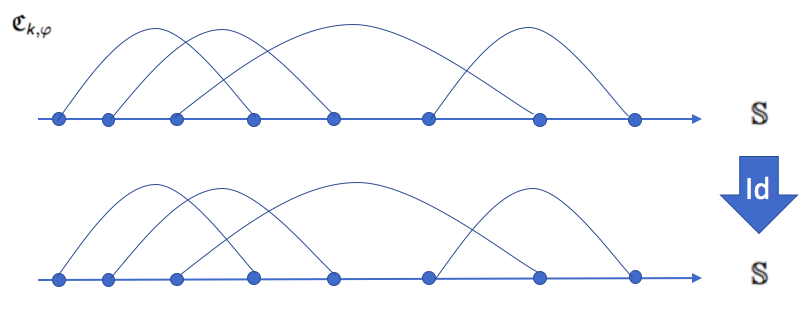
\includegraphics[scale=0.4]{id.png}
}
% gwiazdke na kolko i od lewej do prawej !!!

% Fraisee theory - fraisee category 
\frame{
\frametitle{Morphisms - emmbedings }
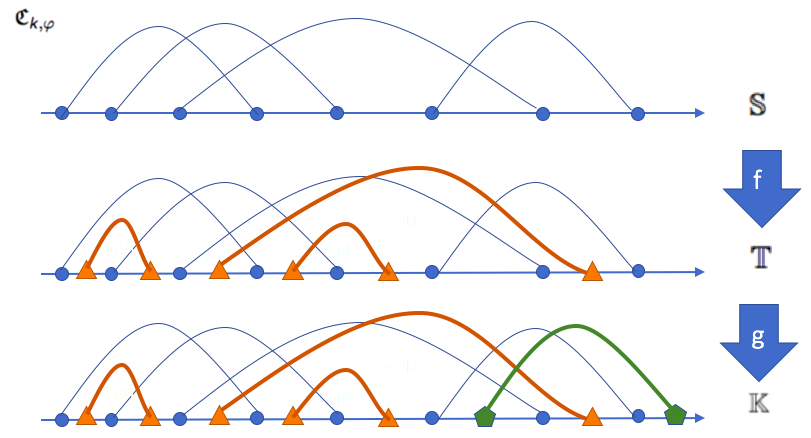
\includegraphics[scale=0.4]{map.png}
}
\frame{
\frametitle{Composition of morphisms}
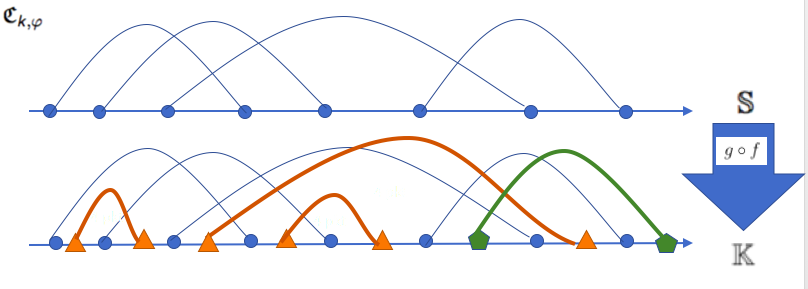
\includegraphics[scale=0.43]{map2.png}
}


\section{Fra\"\i sse limit}

\frame{
\begin{block}{The amalgamation property}
%Each two embeddings can be extended to a further embedding!\\
Given $$f:S\to T, \;  g:S\to K,$$
there should exist an object $W$ and embeddings $f':T\to W$ and $g': K\to W$ satisfying
$$f'\circ f = g' \circ g$$
\end{block}
\begin{block}{}
\begin{center}
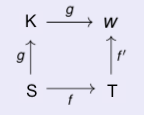
\includegraphics[scale=0.55]{amal.png}
\end{center}
\end{block}

}

\frame{
\frametitle{The chord category as a Fra\"\i sse category example}
\begin{columns}
 \begin{column}{0.4\textwidth}
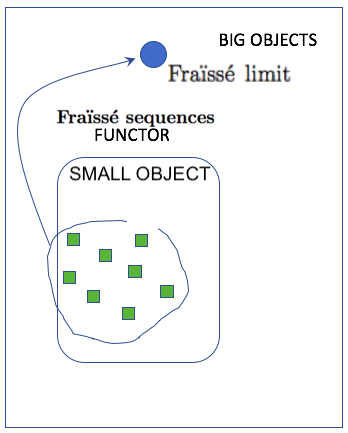
\includegraphics[scale=0.4]{limit.png}
 \end{column} 
\begin{column}{0.5\textwidth}
\begin{block}{Universal chord diagram}
In one backbone case Fra\"\i sse limit is the Rado graph with a linear ordering isomorphic to the rationals.
\begin{center}
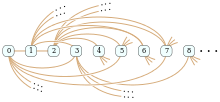
\includegraphics[scale=0.4]{rado.png}
\end{center}
\end{block}
% objects na obrazku !!! 

\end{column}
\end{columns}
 
 
}

\section{Summary}


\end{document}
